%---------------- COMMENT FOR IMPORTING ----------------------
%\RequirePackage{lineno}					%Comment for importing
\documentclass[12pt]{report}		%Comment for importing
%\pagestyle{headings}
%\input{ST-input2}								%Comment for importing
%Usepackages
%\linespread{2}
\linespread{1.3}
%Maths mode programs
\usepackage{amsfonts,amsmath,amssymb,mathrsfs,amsthm}
%Page format									
\usepackage[top=25mm, bottom=25mm, left=25mm, right=25mm]{geometry}	%left = 38mm	
%Figure programs
\usepackage{graphicx}										
%\usepackage[nodayofweek]{datetime}			
\usepackage[authoryear,round]{natbib}
\usepackage{algorithm}
\usepackage{algorithmic}
\renewcommand{\algorithmicrequire}{\textbf{Input:}}
\renewcommand{\algorithmicensure}{\textbf{Output:}}
%\usepackage{algpseudocode}
%\usepackage{tkz-graph}
%\usetikzlibrary{arrows}
\usepackage{xcolor,colortbl}
\usepackage{caption}
\usepackage{subcaption}
\usepackage{subfig}
\usepackage{tabularx}
%\usepackage{cite}
\newtheorem{mydef}{Definition}

\DeclareMathOperator*{\argmin}{arg\,min}
 
\def\Var{{\rm Var}\,}
\def\var{{\rm var}\,}
\def\E{{\rm E}\,}


%macros
\let\oldsection\section
\renewcommand{\section}[1]{
	\setcounter{figure}{0}
	\setcounter{table}{0}
	\setcounter{equation}{0}
	\oldsection{#1}
}

%Ordinal Superscripts
\newcommand{\st}{\textsuperscript{st}~}	%st superscript
\newcommand{\nd}{\textsuperscript{nd}~}	%nd superscript
\newcommand{\rd}{\textsuperscript{rd}~}	%rd superscript
\newcommand{\Th}{\textsuperscript{th}~}	%th superscript

%%Maths Environments
\newenvironment{mat}{\left[ \begin{array}}{\end{array} \right]}
\newenvironment{deter}{\left| \begin{array}}{\end{array} \right|}
\newenvironment{ifbrace}{\left\{ \begin{array}}{\end{array} \right.}

%Table, Equation and Figure Labels
\renewcommand{\thefigure}{\thesection.\arabic{figure}}
\renewcommand{\thetable}{\thesection.\arabic{table}}
\renewcommand{\theequation}{\thesection.\arabic{equation}}

%%Number type
\newcommand{\NN}{\mathbb{N}}	%Natural
\newcommand{\ZZ}{\mathbb{Z}}	%Integer
\newcommand{\RR}{\mathbb{R}}	%Real

%%Statistical Notation
\newcommand{\PP}[1]{\mathbb{P}\left(#1\right)}		%P()
\newcommand{\EE}[1]{\mathbb{E}\left[#1\right]}		%E[]
\newcommand{\VAR}[1]{\mbox{Var}\left(#1\right)}		%Var()
\newcommand{\PiDist}[1]{\pi\left(#1\right)}				%pi()
\newcommand{\cov}[2]{\mbox{Cov}\left(#1,#2\right)}	%Covariance
\newcommand{\corr}[2]{\mbox{Corr}\left(#1,#2\right)}	%Correlation
\newcommand{\Like}[1]{L\left(#1\right)}						%Likelihood
\newcommand{\lLike}[1]{\ell\left(#1\right)}				%log-likelihood

%%Distributions
\newcommand{\Gauss}[2]{\mathcal{N}\left(\quad #1,\quad #2 \quad\right)}
\newcommand{\MVGauss}[3]{\mathcal{MVN}_{#1}\left(\quad #2,\quad #3 \quad\right)}
\newcommand{\IGam}[2]{\mathcal{IG}\left(\quad #1,\quad #2 \quad\right)}
\newcommand{\T}[4]{\mathcal{T}_{#1}\left(\quad #2, \quad #3, \quad #4 \quad \right)}
\newcommand{\dT}[5]{\mathcal{T}_{#1}\left(\quad #2; \quad #3, \quad #4, \quad #5 \quad \right)}
\newcommand{\MVT}[4]{\mathcal{T}_{#1}\left(\quad #2, \quad #3, \quad #4 \quad\right)}
\newcommand{\BETA}[2]{\mathcal{B}\mbox{eta}\left(\quad #1, \quad #2 \quad \right)}
\newcommand{\dBETA}[3]{\mathcal{B}\mbox{eta}\left(\quad #1; \quad #2, \quad #3 \quad \right)}

\newcommand{\Bern}[1]{\mathcal{B}\mbox{ern}\left(\quad #1 \quad\right)}
\newcommand{\Pois}[1]{\mathcal{P}\mbox{oisson}\left(\quad #1 \quad\right)}

%%Mathematical symbols
\newcommand{\half}{\dfrac{1}{2}}												%1/2
\newcommand{\third}{\dfrac{1}{3}}												%1/3
\newcommand{\quarter}{\dfrac{1}{4}}											%1/4
\newcommand{\const}{\! {\rm const.}\; }									%constant
\newcommand{\recip}[1]{\frac{1}{#1}}										%reciprocal - 1/x
\newcommand{\set}[1]{\left\{ #1 \right\} }							%{---}
\newcommand{\seq}[1]{\left( #1 \right)}									%(---)
\newcommand{\e}[1]{{\mbox{exp}}\left\{ #1 \right\}}			%exponent (text)
\newcommand{\Gamm}[1]{\Gamma\left( #1 \right)}				  %Gamma function
\newcommand{\Ind}[1]{\mathbb{I}_{\left\{#1\right\}}}		%Indicator Function
\newcommand{\Id}[1]{{I}_{#1}}														%Identity Matrix
\newcommand{\limit}[2]{\stackrel{\lim }{_{ #1 \to #2 }}}%Limit
\newcommand{\maxover}[1]{\stackrel{\max }{_{ #1 }}}			%max
\newcommand{\minover}[1]{\stackrel{\min }{_{ #1 }}}			%min
\newcommand{\OVec}{\mathbf{0}}													%Zero Vector
\newcommand{\IVec}{\mathbf{1}}													%Ones Vector



%Theorem, Lemma, Proposition, Corollary
\newtheorem{definition}{Definition}[section]
\newtheorem{theorem}[definition]{Theorem}
\newtheorem{lemma}[definition]{Lemma}
\newtheorem{proposition}[definition]{Proposition}
\newtheorem{corollary}[definition]{Corollary}

\newtheoremstyle{mystyle}  % follow `plain` defaults but change HEADSPACE.
  {}   				% ABOVESPACE
  {}   				% BELOWSPACE
  {}  				% BODYFONT
  {0pt}       		% INDENT (empty value is the same as 0pt)
  {\bfseries}	% HEADFONT
  {:}        % HEADPUNCT
  {5pt plus 1pt minus 1pt}				  % HEADSPACE. `plain` default: {5pt plus 1pt minus 1pt}
  {}          % CUSTOM-HEAD-SPEC

\theoremstyle{mystyle}% default
\newtheorem*{eg}{Working Example}

\newenvironment{workedexample}[1]{\begin{eg}\textbf{#1}\\}{\hfill $\blacktriangle$ \end{eg}}

\usepackage[authoryear,round]{natbib}
%\setcounter{chapter}{2}
\begin{document}								%Comment for importing
%\setpagewiselinenumbers
%\linenumbers
%\tableofcontents
%\graphicspath{{figures/}}
%-------------------------------------------------------------

\chapter{Spectral Clustering for Data Streams}


\section{Introduction}

Spectral clustering has been empirically shown to perform well under difficult cluster scenarios, but is computationally intensive to run for large data sets. KASP offers an approach to deal with this burden, by summarising the data using k-means, and feeding the centroids as input to spectral clustering. We show how spectral clustering can be applied to online data by combining the Clustream framework with the concepts developed in KASP \cite{Yan2009}. Clustream is a framework for dealing with a constant stream of data, and splits the clustering process into two stages: micro-clustering and macro-clustering. We analyse the performance of spectral clustering in an online setting on simulated and real texture-based data sets, both for static and evolving streams. We discuss how to quantify the information loss from summarising the data stream and investigate empirically and algebraically how this perturbation may effect the overall performance. 

\section{Literature Review}
\label{sec:spec_lit}


Spectral Clustering is a technique for separating data into many groups or clusters. All the elements in each group should be similar, and elements in different groups should be dissimilar.  A weighted distance matrix of the data points can be formed, which is called an affinity matrix. By evaluating the spectral properties of this affinity matrix, clusters can be determined. This idea of splitting a data set into groups or clusters, with high within-cluster similarity and between-cluster dissimilarity, can also be thought of as a graph partitioning problem, with the data points as graph vertexes, and the elements in the affinity matrix representing weights on the graph edges. Imagine that all of the data points in the data set are joined together by string. If you were asked break this graph into two distinct pieces, which strings would you cut? 

Graph partitioning problems have long been of interest to mathematicians, ever since Euler solved the popular ``Seven Bridges of K\"{o}nigsberg'' problem in 1736. However the link between graph partitioning and matrix spectra was observed much later when \cite{Donath1973} established a lower bound for the number of edges which must be cut in a graph partitioning problem, based on  a factor of the eigenvectors of the affinity matrix. Around the same time \cite{Fiedler1973} published work commenting on the importance of the value of the second eigenvector of the affinity matrix when producing a two way graph partition, also know as a bi-partition. As bi-partitioning was studied the question arose, how to step from bi-partitioning problems to n-partitioning problems? The obvious two approaches are to either recursively apply bi-partitioning on the graph or calculate an n-partition directly from the first $n$ eigenvectors. This is discussed further in \cite{Alpert1995} where they claim that recursive bi-partitioning, which was more popular at the time, is inferior compared with creating one partition using many eigenvectors. For a full review of the historical origins of spectral clustering, see the tutorial \cite{Luxburg2008}.

The first paper to really highlight the use of Spectral Clustering to the Machine Learning community came in 2000. \cite{Malik2000} treated image segmentation as a graph-cut problem. Mathematically, a cut of a graph G is the set of edges S, such that the removal of S from G disconnects G. A graph is connected if there is a path from every vertex to every other vertex in G. The weight of the cut can be calculated by summing the weights of the edges which will be broken when a cut is made, as given in equation \eqref{eq:cut}. 


\begin{equation}
  \text{cut(A,B)} = \sum_{p \in A, q \in B} w(p,q)
  \label{eq:cut}
\end{equation}

The Minimum cut proposed in \citep{Wu1993} is simply the cut which generates the minimum cut weight. However the  minimum cut does not always provide the best solution; it tends to favour removing small sections and isolated nodes of the graph.  The main proposal from Malik was to consider the cut function as a fraction of the total edge connections to all nodes in the graph, instead of using the total edge weight connecting the two partitions. This subtle yet important distinction provides us with the highly acclaimed normalised cut (NCut), defined in equation \eqref{eq:ncut}, which is an integral part of spectral clustering algorithms.  The main idea is that big clusters will increase assoc(A,V), thus decreasing Ncut(A,B).  Minimising the normalised cut is an NP-complete problem but an approximate solution can be found efficiently by finding the eigenvector with the second smallest eigenvalue. 
  
\begin{eqnarray}
  \text{Ncut(A,B)} &= \frac{\text{cut(A,B)}}{\text{assoc(A,V)}} + \frac{\text{cut(A,B)}}{\text{assoc(B,V)}} \\
  \text{assoc(A,V)} &= \sum_{u \in A, t \in V}w(u, t) \nonumber
  \label{eq:ncut}
\end{eqnarray}

On Spectral Clustering \cite{Ng2001} was one of the first papers to provide theoretical guarantees on performance for spectral clustering algorithms.  Unlike previous authors who had only shown empirical results to justify spectral clustering abilities, they prove that their spectral clustering algorithm will produce a reasonable clustering, given certain assumptions that the clusters are well-spaced. %This version of the spectral clustering algorithm has been popularly cited throughout the literature and indeed it is the one that we shall reference in Section \ref{sec:spec}. 

Although spectral clustering has been shown to perform well empirically on simple data sets, computational problems arise as the data set size increases. There have been a number of ways to deal with speed up in the static case, one of the most popular methods is to use Nystr\"{o}m efficiency methods \cite{Williams2001} \cite{Fowlkes2004}. The Nystr\"{o}m method samples the columns of the affinity matrix and approximates the full matrix by using correlations between the sampled columns and the remaining columns. 

An alternative to Nystr\"{o}m methods is to perform some data permutation on the data as a pre-processing step. By feeding a smaller set of representative points into the spectral clustering algorithm instead of the whole data set, we can lessen the effect of the computations bottleneck that comes with eigen analysis. Fast Approximate Spectral Clustering \cite{Yan2009}, \cite{Huang2009} explores the theoretical guarantees on misclustering the data set, given that some permutation has been performed on the data before the spectral clustering. Specifically they exactly quantify the misclustering of data sets, given that the original data is summarised using K-means (KASP) or a Random Project tree (RASP) as preprocessors. 

Another recent improvement to deal with the computational issues in spectral clustering is proposed in Local Information-based fast approximate spectral clustering \cite{Cao2014}. Li-ASP consists of two upgrades a sparse affinity graph to speed up computation and local interpolation to improve clustering performance. The sparse affinity graph effectively uses $k$ nearest neighbour or an $\epsilon$ neighbourhood to set many elements in the affinity graph to 0. Local interpolation is suggested based on an issue identified about KASP \cite{Yan2009} that if a representative point is miss-assigned to the wrong cluster, then all members of that cluster will be miss-assigned. Local interpolation can avoid these situations by using weighted differences from the nearest $p$ centres that a data point belongs to. KASP only uses it's assigned cluster. 

The choice of scaling parameter $\sigma$ is discussed in \cite{Zelnik-Manor2004}. They argue that for data which has a cluttered background, or multi-scale data, one global parameter choice for $\sigma$ is not sufficient. Before this, the most common method for choice of parameter was manually or \cite{Ng2001} automatically chose $\sigma$ by running their clustering algorithm repeatedly for a number of values and selecting the one which provides least distorted clusters of the rows of $Y$. In \cite{Zelnik-Manor2004} a localised parameter is calculated. Each data point has it's own $\sigma$ value calculated based on it's neighbourhood (here $K = 7$). They also present a method for automatically choosing the true number of clusters $C$ using the eigenvectors to inform a choice. More commonly the eigenvalues are commonly used to estimate $K$ but if the groups are not clearly separated, identifying the number of groups from eigenvalues alone is not trivial. 


%The above cluster static data sets. We are interested in data streams, which are of great interest in today's world of communication graphs such as the internet and social networks. Applications also include health care such as modelling epidemics and security issues - understanding sensor networks. We could re-cluster the graph at each time step whenever new information arrives but this can be inefficient and computationally expensive, especially if data is arriving rapidly. Continuously generated data - unsupervised learning. What are the challenges: non-stationary, unbounded data. Algorithms should be fast. Random Access is expensive (Guha 2003) therefore do linear scans.  Review paper \cite{Silva2013}. Birch \cite{Zhang1996a}. Clustream \cite{Aggarwal2003}

%Most methods assume finite amount of data generated by unknown stationary probability distribution. The restrictions for data stream noted in \cite{Silva2013} are data objects arrive continuously. There is no control over the order in which data objects should be processed. The size of stream is potentially unbounded. Data objects are discarded after processing (or stored for short period and use a forgetting mechanism).  The unknown underlying data process is possibly non-stationary. We want to determine a finite set of clusters which describe the data set.  Fayyad 1996 - objects within a cluster are more similar to each other than they are to objects belonging to a different cluster. Cao 2006, Yanh Zhau 2008 Zhou 2008. Split object-based data stream clustering algorithms into two main steps, data abstraction (online) and clustering (offline)

% \cite{Valgren2007} Work on topological mapping. Incrementally updates the affinity matrix to deal with large data sets. Issues include that the number of overall clusters $C$ must always increase.

 \cite{Ning2007} \cite{Ning2010} Updates eigenvalues incrementally. A change in vertices or edge can be used to algorithmic-ally update the eigenvalues and eigenvectors directly, however the authors recommend a full re-clustering in batch to minimise cumulative errors. The indirect updating of eigenvectors means that the orthogonality property may be lost. Also if the spatial neighbourhoods of often changing vertices are large it can still be computationally hard as the eigenvalue step involves the inversion of a matrix.
% \cite{Kong2011} Used un-normalised and representative points like \cite{Yan2009}. Solution updated when vertices change but not the edges. \cite{Dhanjal2014} Online graph clustering developed Incremental Approximate Spectral Clustering using SVD based on \cite{Dhanjal2011}. We propose an online spectral clustering algorithm based on the Clustream model. \cite{Aggarwal2003}  Lead into other relevant online data clustering papers.  

%\cite{Kannan2004} \cite{Cao2014} \cite{Dhanjal2014} \cite{Guattery1998} \cite{Hagen1992} \cite{Jordan2004} \cite{Huang2009} \cite{Meila2001} \cite{Ng2001}  \cite{Pothen1990}  \cite{Stoer1997} \cite{Tibshirani2001} \cite{Luxburg2005} \cite{Luxburg2007} \cite{Wu2014} \cite{Yan2009} \cite{Zelnik-Manor2004} \cite{Zhang2014} \cite{Valgren2008}
%\begin{quote}
%``Image partitioning is to be done from the big picture downward, rather like a painter first marking out the major areas an then filling in the details.'' - Jianbo Shi and Jitendra Malik
%\end{quote}
%\cite{Malik2000} in relation to image segmentation structure leading to hierarchical solutions - not a final solution.



\section{Spectral Clustering}
\label{sec:spec}

In this Section we provide a brief introduction to Spectral Clustering, and discuss the choice of affinity matrices. The KASP \cite{Yan2009} algorithm will be introduced, which we will use in an online fashion in Section \ref{sec:microSpec}.

The goal of spectral clustering is to partition the data  into $k$ disjoint classes such that each $x_i$ belongs to one and only one class. Data which is compact may be simple to cluster as the gaps between clusters are easier for simple clustering algorithms to identify. Sometimes data may be connected and therefore should hopefully be classed as a whole cluster, but it may not be tightly compact and spherical. Spectral clustering can provide good quality segmentation on even these difficult cases, however its performance comes at the cost of computational complexity. We shall use the Jordan-Weiss (NJW) spectral clustering framework \cite{Ng2001} which is described in Algorithm \ref{alg:njw}. 

We want to use a matrix to represent the pairwise similarities or distances between all data points $i$ and $j$, called $a_{i,j}$.  We refer to the matrix $A = (a_{ij} )_{i,j = 1}^n$ as the affinity matrix.  We can think of the affinity matrix $A$  as a metric that determines how close two points are in our space. A popular choice is to define $A$ to be the Gaussian kernel, as defined in equation \ref{eq:gaussian_affinity}, where the parameter $\sigma$ controls the width of the local neighbourhoods which we want to model.
\begin{equation}
  \label{eq:gaussian_affinity}
    a_{i,j} = \exp  \left( - \frac{\| x_i - x_j \|^2}{2 \sigma^2} \right), i, j = 1, \ldots, n.
\end{equation}
 If $x_i$ and $x_j$ are very close, then $a_{i,j} \rightarrow 1 $, and if they are far apart $a_{i,j} \rightarrow 0$. This matrix will have ones along the diagonal, and will be symmetric ($a_{ij} = a_{ji})$.

If we mainly wish to model the local relationships, using all of the possible pairwise data connections may not be necessary. It is possible to use a weighted k-nearest neighbour structure to build the affinity matrix (once corrections have been made to ensure that this matrix is symmetrical). Another option is to choose some threshold $\epsilon$ and only consider connections between data points whose pairwise distances are smaller than $\epsilon$. This is an $\epsilon$-neighbourhood graph. Although we can weight by $\epsilon$, if we choose $\epsilon$ to generate a small $\epsilon$-neighbourhood, then the differences between the weights will be small/negligible. Therefore a simple construction of the $\epsilon$-neighbourhood graph is as follows. 

\begin{equation}
  a_{ij}=\left\{
  \begin{array}{@{}ll@{}}
    1, & \text{if}\ d_{ij} < \epsilon \\
    0, & \text{otherwise}
  \end{array}\right.
\end{equation} 

Using this construction would give a sparse affinity matrix instead of a fully connected graph, which will help lower the computational complexity. 

 The degree of each vertex $v_i$ is defined as, $d_i =\sum_{j = 1}^N A_{ij}$, the sum of the rows of the affinity matrix. The degree matrix, $D$, is then defined as a diagonal matrix with $i$\textsuperscript{th} diagonal element equal to $d_i$. We use the Normalised Laplacian defined in equation \ref{eq:norm_laplacian}, which relates to an approximation of minimising the Normalised Cut, discussed in Section \ref{sec:spec_lit}. Ideally, the Laplacian $L$ will be block-diagonal, where each block refers to a particular cluster. 

 \begin{equation}
   \label{eq:norm_laplacian}
   L=D^{-1/2}AD^{-1/2}
 \end{equation}


\begin{algorithm}
\caption{NJW spectral clustering algorithm}
\begin{algorithmic}[1]
\REQUIRE Data set $S = {x_1,\ldots, x_n  }$, number of clusters $k$
\ENSURE $k$-way partition of the input data
\STATE Construct the affinity matrix $A$ by the following Gaussian kernel function:
\begin{equation*}
  a_{i,j} = \exp  \left( - \frac{\| x_i - x_j \|^2}{2 \sigma^2} \right), i,j = 1, \ldots,n.
\end{equation*}

\STATE Compute the normalised affinity matrix $L = D^{-\frac{1}{2}}A D^{-\frac{1}{2}}$, where $D$ is the diagonal matrix with $D_{ii}=\sum_{j=1}^{n} a_{ij}.$
\STATE Compute the $k$ eigenvectors of $L$, $v_1, v_2,\ldots , v_k,$ associated with the $k$ largest eigenvalues, and form the matrix $ X = [v_1,v_2, \ldots , v_k]$.
\STATE Renormalize each row of $X$ to form a new matrix $Y$.
\STATE Partition the $n$ rows into $k$ clusters via a general cluster algorithm, such as the k-means algorithm.
\STATE Assign the original point $x_i$ to the cluster $k$ $\iff$ the corresponding row $i$ of the matrix $Y$ is assigned to the cluster $k$.

\end{algorithmic}
\label{alg:njw}
\end{algorithm}

Spectral clustering can be challenging for very large data sets, constructing the affinity matrix $A$ and computing the eigenvectors of $L$ have computational complexity $\mathcal{O}(n^2)$ and $\mathcal{O}(n^3)$ respectively. \cite{Yan2009} proposes a fast approximate spectral clustering which uses a k-means pre processing step to lessen the computational complexity whilst retaining good clustering performance. Firstly k-means is run on the whole data set where $k$ is chosen to be large but such that $k \ll n$. The centres of the clusters are then used as representative data points for the whole data set. Spectral clustering is performed on the representative set only, which is faster than performing spectral clustering on the full data set. The resulting cluster labels for the representative data are linked back to the original data set such that every original data point acquires the same label as its associated $k$-means cluster center. The KASP algorithm is repeated in Algorithm \ref{alg:kasp} with modified notation.

\begin{algorithm}
\caption{KASP}
  \begin{algorithmic}[1]
   \REQUIRE $n$ data points $\{xi\}_{i = 1}^n$, number of representative points $k$
   \ENSURE  $m$-way partition of the input data
   \STATE Perform k-means with k clusters on $x_1, \hdots, x_n$ to:
   \STATE a) Compute the cluster centroids $y1, \hdots, y_k$ as the $k$ representative points.
   \STATE b) Build a correspondence table to associate each $x_i$ with the nearest cluster centroids $y_j$ .
   \STATE Run a spectral clustering algorithm on $y_1,\hdots, y_k$ to obtain an $m$-way cluster membership
   for each of $y_i$.
   \STATE Recover the cluster membership for each $x_i$ by looking up the cluster membership of the corresponding centroid $y_j$ in the correspondence table.
  \end{algorithmic}
\label{alg:kasp}
\end{algorithm}

\section{Micro-cluster based spectral clustering in data streams}
\label{sec:microSpec}

A relatively new challenge to clustering is working with data streams. Data stream clustering is clustering of data which arrives in an ordered sequence, continuously; for example, sensor data or shopping transactions. Much work has been done developing offline clustering methods, such as spectral clustering, but it is not suitable to apply these offline methods to the streaming scenario. Simply running an offline clustering algorithm on all the data observed so far may not be feasible. Often, the data cannot be stored in its entirety, therefore the older data has to be thrown away to make room for the new arrivals. This might at first seem like not a big issue as this will naturally weight the data temporally. However we may still wish to use older data in current clustering. Also clustering algorithms can be computationally expensive. For example, spectral clustering has $\mathcal{O}(n^3)$ when solving the eigenvalue problem. Therefore we need to be able to update our idea of the data as new points arrive efficiently and simply with little computational issues. Also we have the issue that we will only see the data once (one-pass). This can be imagined as data flying past in a chute. You can look at the data as it flies by, but once it has passed by, it cannot be accessed again. Some algorithms such DBScan require many passes or iterations of the data, therefore these type of clustering methods are not directly suitable for the online data streaming case. 

Clustream \cite{Aggarwal2003} offers a framework which allows quick and easy updates and the ability to perform sophisticated clustering algorithms. The main idea is to separate the clustering process in two stages;  a micro clustering which continuously updates statistical summaries of the data set, and a macro clusterer which is run on a user request. The micro-clusters are defined as a temporal extension of the cluster feature vector \cite{Zhang1996a}. 

Assume that we have a data stream $S$ which consists of $d$-dimensional data $x_i$ arriving in sequence. $S = \{ x_1, x_2, x_3, \hdots x_i, \hdots, \}, x_i \in \mathbb{R}^d$ 

Keeping track of all of the data is very hard. As we have mentioned above, we only have one-pass access to the data. This is where the idea of micro clusters comes in. Micro clusters are a way of maintaining an active, evolving representative summary of your data, without actually having to store the absolute values for all the data points. This data summary can then be used on a user request to perform a macro clustering using the summarised data rather than the full data set. If the micro clusters represent the true underlying data stream well, then the difference between the clustering on the summarised data and the true full data should be small. This was shown in \cite{Yan2009}. 

How does this micro-clustering work? The data stream is summarised by many small clusters, which are initially generated by k-means. We take an initial training set, and perform k-means but choose the value of $k$ to be much larger than the expected number of true macro clusters. The aim here is to create a fine scale summary of the data. The value of $k$ should be chosen to be as large as computationally comfortable. The larger $k$ is, the finer scale that the summaries will be. It is vital to ensure that the micro-cluster well represent the underlying data set or else the macro clustering will under perform. 

These $k$ clusters are our first micro clusters. Over time, we will update these micro clusters. Adding new data points to them, and sometimes removing old micro clusters to make the way for new micro clusters (the number of micro clusters should stay fixed throughout). 

Each micro-cluster $j$ is stored as a ($2 \cdot d + 3$) tuple $(CF1^x, CF2^x, n, CF1^t, CF2^t)$. $CF1^x$ is the sum of all observed data in that micro cluster, $CF2^x$ is the sum of the squares of the data and $n$ is the number of elements in the micro-cluster. $CF1^t$ and $CF2^t$ refer to the sum of the time stamp, and the sum f squared time stamps respectively. 
Note that both $CF1^x$ and $CF2^x$ will have $d$ entries, one for each dimension.

Micro-cluster $j$ will have 
\begin{align*}
CF1^x[p] = \sum_{x_i \in j}{x_i^p},   \\
CF2^x[p] = \sum_{x_i \in j}{(x_i^p)^2}.
\end{align*}

These updates only require addition therefore they are cost effective. Critically it is possible to use these summaries to calculate the centre of each micro-cluster. It is these centres which as used as representative points for input into the macro clustering.  As new points in the data stream arrive, they are either allocated to a micro-cluster and the update procedure discussed above it carried out, or a new micro-cluster is created. The decision for a new micro cluster to be created is based on whether the new data point is close enough to it's nearest cluster centre. 

When a new data point arrives, it's nearest micro-cluster is identified using the Euclidean distance metric. If the data point falls within the Maximum Boundary Factor of it's nearest cluster centre, then it is absorbed as part of that cluster. If not, it is used to create a new micro-cluster. However we stated earlier than the number of micro-clusters must remain fixed throughout the process. Therefore if a new micro-cluster is formed, either an existing  micro-cluster must be deleted, or two close micro-clusters should be merged. We follow the methodology in Clustream by first looking for an ``old'' micro-cluster to delete (using the time-stamp references detailed in the original paper) and otherwise combine the two nearest micro-clusters. In this way, the algorithm should be able to track the data stream as it evolves. 

With this online micro-cluster maintenance, the data stream should remain well represented over time. When a new data point arrives, if it is the start of a new evolving cluster, it will be allowed to grow, however if it is an outlier, no more points will be added to it, and over time it may be deleted from the system all together.

Clustream has proved popular over time. Since the paper was first published in 2003, it has been cited over 1400 times. Empirically there is much evidence to show that micro-clustering is an effective way to maintain information about your data set. However there has been little theoretical work to explain why this micro-clustering method seems to work so well. 



%In this section, we discuss the similarities between the micro-clustering stage, and Gausssian Mixture Models. We describe the update proceedure in the framework of an online Expectation Maximisation Algorithm for Gaussian Mixture Models, and discuss the assumptions required to make this work. 


%A Gaussian mixture model is a model which consists of the combnination of a number of Gaussians distributions. We can imagine that the datapoints are drawn from one of o the Gaussian distriubtions randomly, according to some mixture probability $/pi$. 
%In the simplest case, we could have a Gaussian mixture model with 2, components, each with a probability of $\frac{1}{2}.$

%In micro-clustering, the boundaries are chosen to be the a factor of the quadratic mean from the center of the cluster.

%Thhe expectation-maximasation algorithm is required to 

%For the online case, an online expectation maximsation algorithm exists. Infact a couple fo possibles exist. 

%Each time a new data-point is observed, firstly the mixture probability vector $\pi$ is updated, and then the components of the multivariate Guassian mixture distributions $\mu_1, \hdots, \mu_k$, and $\sigma_1, \hdots, \sigma_K$ are updated.

%In Clustream, when a new point is identified as belongingto a cluster, it's clsuter centre (the mean) is updated to include that point. 

%What assumptions are we making about the standard deviation in clustream. We assume that it is fixed for all dimensions - aka it is spherical in the feature space. 

Our intention is to a develop method for applying spectral clustering to a data stream. In order to achieve this we adapt a micro-clustering type approach to quickly update a summary of the data. When an overall clustering is required, spectral clustering is performed using the centres of the micro-clusters as the input data. The micro-clusters act as a way of summarising the constantly arriving data steam whilst allowing updates to occur in a non intrusive, non-computationally difficult manner, with limited storage requirements. 

Our algorithm is as follows: 

\begin{algorithm}
\caption{}  
\begin{algorithmic}
\STATE  Initialise micro-clusters
\STATE New data point arrives, update micro-clusters in the manner discussed. Either allocate the data point to an existing micro-cluster or initialise a new micro-cluster. 
\STATE At certain intervals take the centres of the micro-clusters as input to a spectral clustering algorithm. 
\STATE Then link the spectral clustering output back to the original data points (if required) either simply by assuming that each cluster member takes the same result as its cluster centre, or a more complicated weighted method. 
\end{algorithmic}
\end{algorithm}

How should we use the centres as input into spectral clustering? \cite{Silva2013} suggests two ways of using the centres as input; use them directly, or scale them by the number of elements in a micro cluster. The nature of this algorithm allows the user to get close to online streaming and perform spectral clustering on a summary of the whole of the data set.


\section{EM as a micro clustering technique}

\section{Experimentation}
 \label{sec:clust_study}

\section{Conclusion}



%\begin{figure}[h]
%  \centering
%  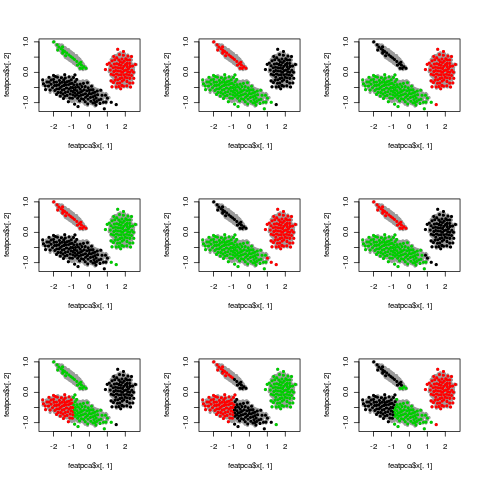
\includegraphics[width = 11cm]{nnSim.png}
%  \caption{When spectral clustering goes wrong - Neighborhood choice - not trivial!}
%\end{figure}



% We wish to see if its possible to get sensible spectral clustering in an online setting.  In order to test this, a number of simulated datasets are used to assess performance. The same online micro-clustering will be used, and then at batch points the macro clustering is performed. The algorithms used for the macro clustering are kmeans, dbscan and spectral clustering. Performance metrics are taken for purity and V-measure. DBScan has chosen parameters, minimum points and epsilon in accordance with suggestion from \cite{ester1996}. 
% The initialisation of microclusters generated by performing k-means on an initial trial dataset consisting of the first datapoints. 

% \subsection{Stationary Datastreams}
% The online clustering is tested when datastream is stationary and non-stationary. Firstly we consider the stationary case. In this setting, the initial trial dataset includes some datapoints from each of the underlying clusters. Throughout the stream, datapoints from these initial clusters are generated. No clusters are removed, merge or join through the dataset. 
% Results are shown for two simulated datasets and one real image based dataset. Dataset A of 2 dimensions, 6 clusters and is normally correlated with uniform mean shift. Dataset B has 8 clusters, and 5 dimensions. Dataset C is  LS2W texture data taken from the KASP dataset. The KASP dataset is a texture database of many different images. I have used a subset of images from this set. The features come from L2SW decompostion for 7 levels in 3 directions - therefore 21 dimensions. I have found that LS2W representation is good at distinguishing between the different textures. 
% PCA plots of all three datasets can be seen in Figure .

% \begin{figure}
%   \centering
%   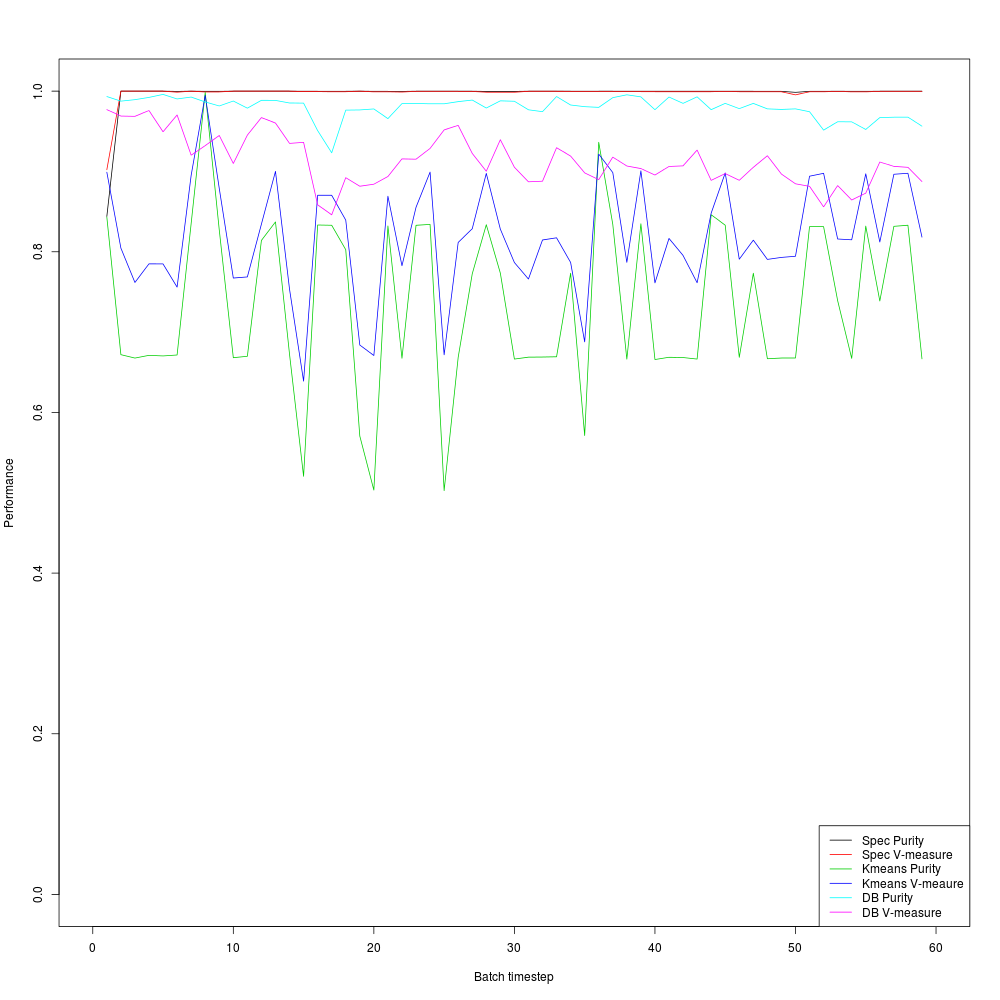
\includegraphics[width = 11cm]{set456.png}
%   \caption{Seed 456, 6 clusters, 2 dimensions - easy}  \label{fig:dataA}
% \end{figure}


% \begin{figure}[h]
%   \centering
%   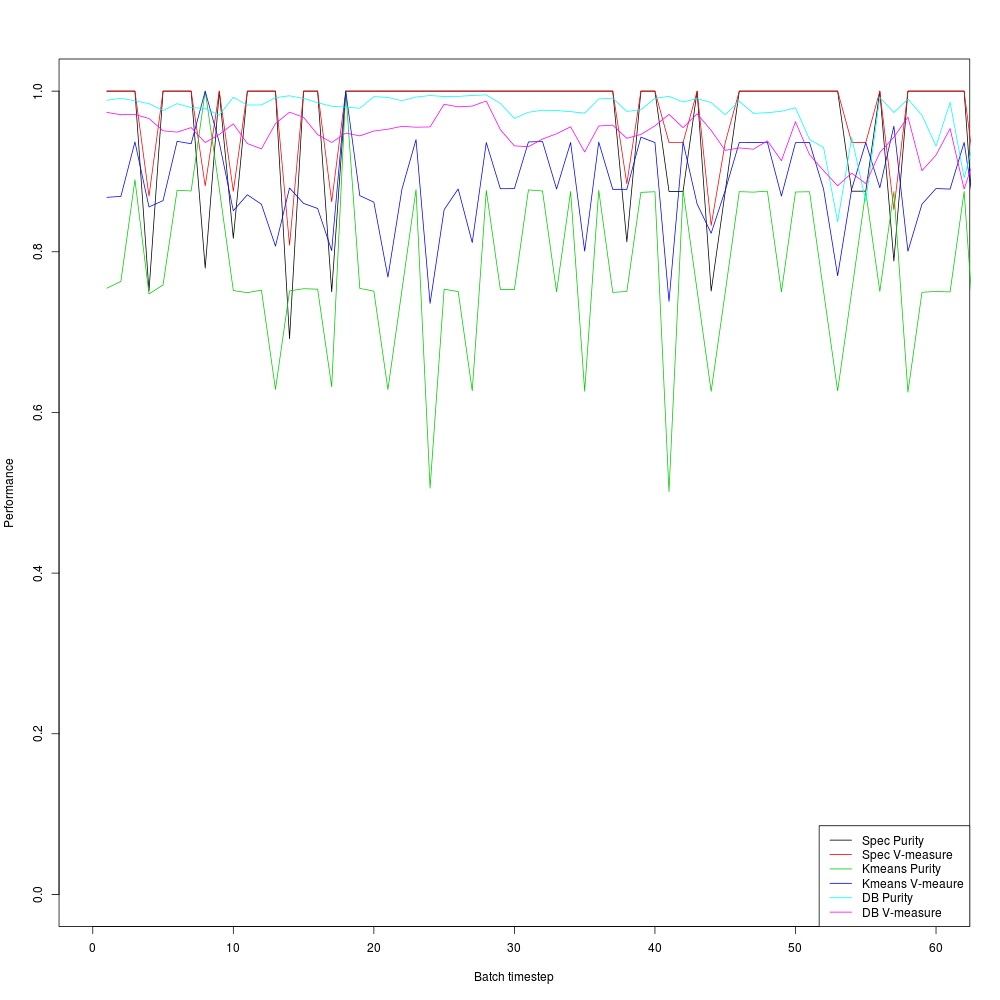
\includegraphics[width = 11cm]{set420.png}
%   \caption{Seed 420, 8 clusters, 5 dimensions - medium} \label{fig:dataB}
% \end{figure}


% \begin{figure}[h]
%   \centering
%   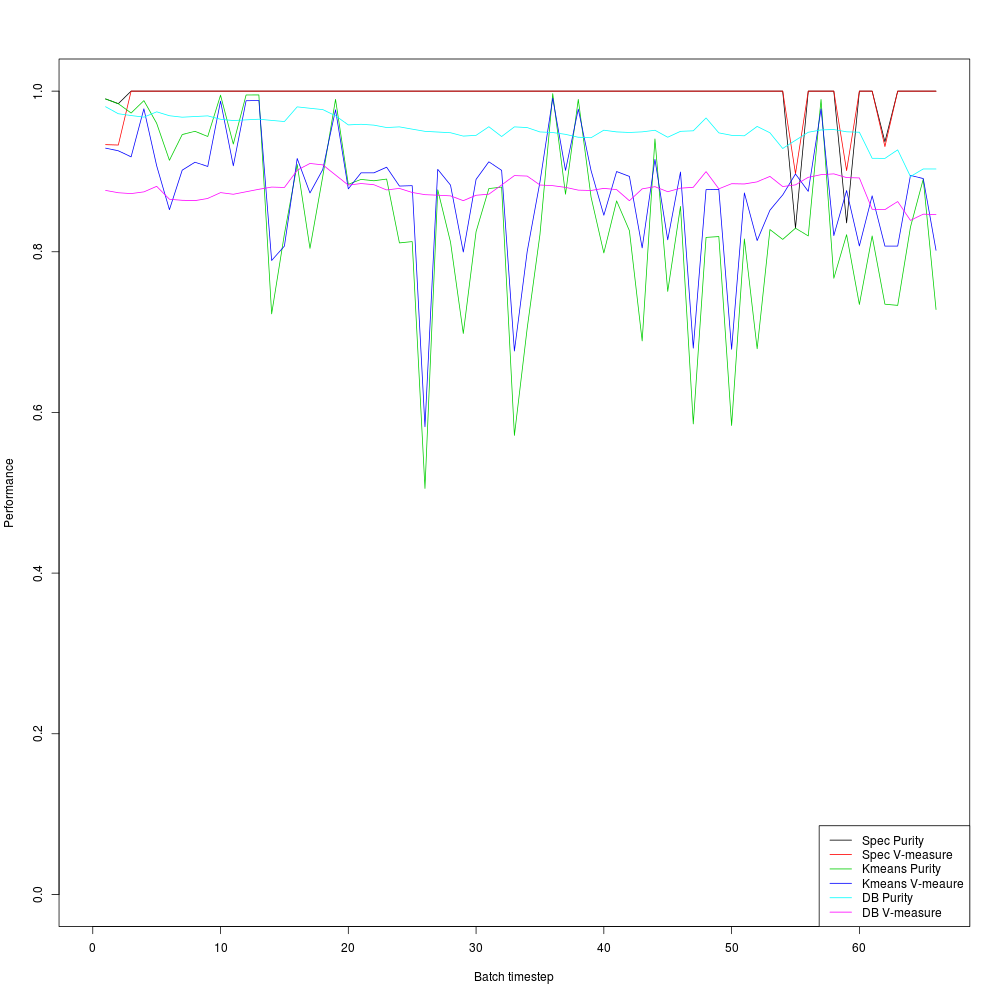
\includegraphics[width = 11cm]{texturebatch.png}
%   \caption{Real texture data, tricker but too short?}
% \end{figure}

% Figure \ref{fig:dataA} shows performance and V-measure for Dataset A over runs of the data. The dataset consists of 60,000 datapoints, and the offline algorithms performed clustering every 1000 timesteps. 250 microclusteres were used to track the datastream. We can see that Kmeans generally performs poorly, jumping around 0.8. DBScan has a more consistant performance, hovering around 0.9. Spectral clustering performs very good segmentation throughout the trial, consistantly having values of 1 for purity and v-measure which corresponds to perfect clustering. We would expect to see this variability in kmeans due to the dependency on the initial seed points.

% Figure \ref{fig:dataB} shows performance and V-measure for Dataset B over runs of the data. The dataset consists of 80,000 datapoints, and the offline algorithms performed clustering every 1000 timesteps. 250 microclusteres were used to track the datastream. We can see that Kmeans generally performs poorly, jumping around 0.8. DBScan has a more consistant performance, hovering around 0.9. Spectral clustering performs perfrect clustering in 52/60 of the clusterings which occasionally drops to 0.9. 

% \subsection{Non-stationary Datastreams}

% Tracking microclusters for non-stationary datastreams brings an additional challenge. Underlying clustering may vanish over time, or move , or new clusters can join. Interesting challenges include succesfully detecting between an outlier of an existing cluster, and the start of a new emereging cluster. 


% \subsection{Time improvement against offline methods}

% Offline spectral clustering. This is standard spectral clustering algorithm performed on all of the most seen data up to time $t$, performed whenever $t$ is divisible by the batch size $b$. As this uses all of the datapoints it can produce very accurate results but is very slow to run. 

% Offline K-means. Standard kmeans, performed on all data up to time $t$ when $\frac{t}{b}$ divides exactly. Very quick but variable performance.

% \begin{figure}[h]
%   \centering
%   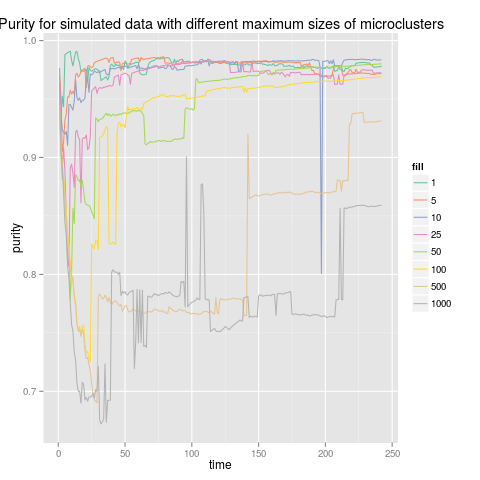
\includegraphics[width = 10cm]{purityMaxMicroClust}
%   \caption{Graphs etc. here}
% \end{figure}

% \begin{figure}[h]
%   \centering
%   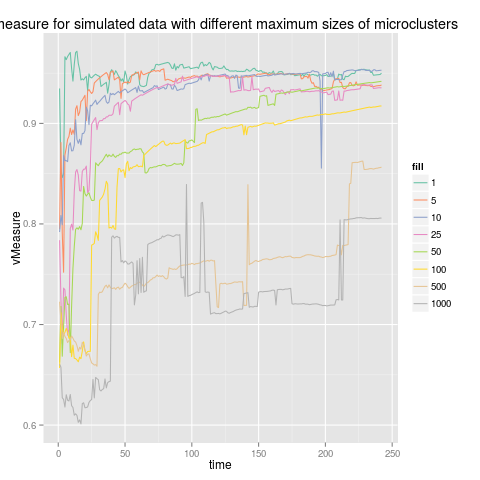
\includegraphics[width = 10cm]{vMeasureMaxMicroClust}  
%   \caption{V measure}
% \end{figure}


% \subsection{Performance Metrics}

% In order to investigate the performance of our algorithm we will assess it on both simulated and real data.  Standard offline spectral clustering will be compared against the streaming spectral clustering. The affinity matrix will be used as described in Section \ref{sec:spec}. V-measure and purity will be used to interpret cluster performance, and specifically a misclustering rate will be used to compare directly against the offline case.  

% introduces the misclustering rate to quantify the difference between an original and perturbed dataset described as 
% \begin{equation}
%   \label{eq:misClust}
%   \rho = \frac{1}{n} \sum_{i = 1}^{n} \mathbb{I}(I_i \neq \tilde{I}_i)
% \end{equation}

% Here $\mathbb{I}$ is the indicator function, $I_i$ represents the cluster allocated to original datapoint $x_i$ and $\tilde{I_i}$ represents the cluster allocation of perturbed datapoint $\tilde{x}_i$. If $\rho = 1$ then the clustering of the perturbed data is identical to the clustering of the original data. In Section \ref{sec:bounds} we will attempt to justify bounds on the values of the misclustering $\rho$ given some understanding of the micro-clustering process used.

 
% To compute purity , each cluster is assigned to the class which is most frequent in the cluster, and then the accuracy of this assignment is measured by counting the number of correctly assigned documents and dividing by $N$. Formally:
% \begin{equation}
% \mbox{purity}(\Omega,C) = \frac{1}{N} \sum_k \max_j \vert \omega_k \cap c_j\vert
% \end{equation} 	
% where $\Omega = \{ \omega_1, \omega_2, \ldots, \omega_K \}$is the set of clusters and $C = \{ c_1,c_2,\ldots,c_J \}$ is the set of classes Bad clusterings have purity values close to 0, a perfect clustering has a purity of 1 .Purity can become very high when there are a large number f clusters and therefore there it is not suitable for all cases, despite its nice simplicity. The V-Measure (A. Rosenberg and J. Hirschberg, 2007.) is described the harmonic mean of the homogenity and the completeness. This allows. Both these measures will allow us to compare the overall performance of the clustering given we know the ideal clustering scenario. However when working online with massive datasets we may be h
% appy to just get a performance as good as or as close to the offline performance as possible

% \section{Theoretical Guarantees and Bounds}
% \label{sec:bounds}
% Aim is to investigate the impact of clustering performance of perturbation on the data. The data perturbation is modelled as noisy observations. 

% $\tilde{x_i} = x_i + \epsilon_i$

% KASP investigated the relationship between data perturbation and the misclutering rate $\rho$ and determined a link between the perturbation on the Laplacian matrices and $\rho$, which is reprinted here. 

% Assume that: 1) the assumptions of Theorem 1(list) hold throughout the recursive invocation of the Ncut algorithm, 2) the smallest eigengap
% $g_0$ along the recursion is bounded away from zero, and 3) the Frobenius norm of the perturbation on Laplacian matrices along the recursion is bounded by $c\|\tilde{L} - L\|_F^2$ for some constant $c \geq 1$. Then the mis-clustering rate for an m-way spectral clustering solution can be bounded by

% \begin{equation}
%   \label{eq:KASPThm3}
%   \rho \leq \frac{m}{g_0^2} \cdot c \| \tilde{L} - L \|_F^2.
% \end{equation}

% This provides a link between the perturbation of the original dataset and the perturbation of the Laplacian matrix. 

%\begin{itemize}
%\item Build in more of existing theory
%\item Discussion of required assumptions
%\item Construct a model structure for the micro-clustering stage
%\item Manual contribution of kmeans effect on very simple case
%\item evolution of the ``frobenius vector'' simple case - what intuituion?
%\end{itemize}








%---------------- COMMENT FOR IMPORTING ----------------------
%\pagebreak											%Comment for importing
\bibliographystyle{plainnat}		%Comment for importing
%\bibliography{References}				%Comment for importing
\bibliography{library, rhian}
\end{document}									%Comment for importing
%-------------------------------------------------------------



